\begin{figure}
    \centering
    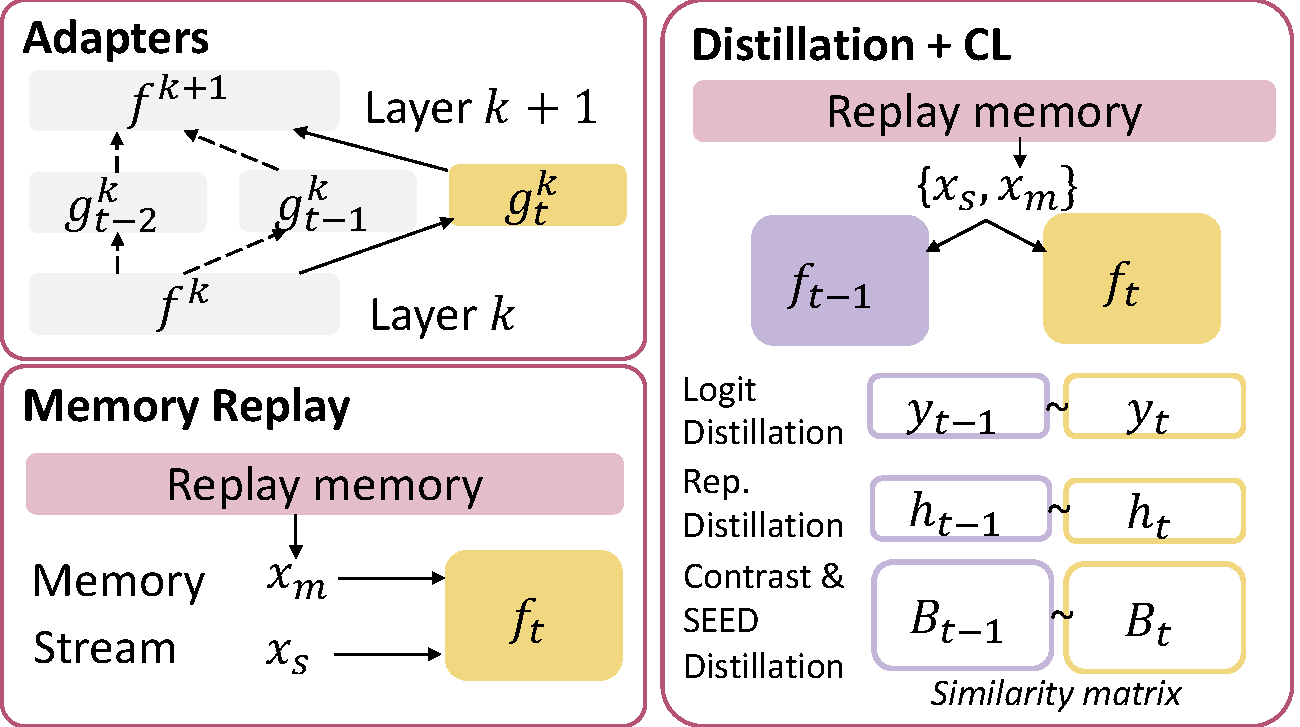
\includegraphics[width=\linewidth]{acl2022/figs/method.pdf}
    \caption{\textbf{Comparison of adapter, memory replay, and distillation-based continual learning algorithms.} 
    Details of the methods are introduced in Sec.~\ref{sec:methods}.
    %We use $g_{t}^k$ to represent adapters created for the task $t$. $\bm{x}_m$ and $\bm{x}_s$ note for the mini-batch of examples drawn from the memory and the data stream respectively.
   % \xiang{Good to include illustration on the three simple baselines.}
    }
    \label{fig:method}
\end{figure}